        This section will make a resume about what's this project about, commend which where the motivation that bring
        me to carry on this project, how to implement it and use it, alongside with how to modify its behaviour.
        With the intention to make reader able to implement and configure it at its desire following simple and
        concise steps while providing a deep understanding of the followed actions.

    \newpage
%    Description
    \subsection{Description}\label{subsec:Description}

        This project is intended to facilitate implementing an online shop with a base infrastructure.
        Offering the capability of:
        \begin{itemize}
            \item Infrastructure based on dockers.
            \item Default web with simple configuration.
            \item Defined database structure.
            \item Backup automation to a local drive or remote server.
            \item Automatic error management among the web-database relation limiting the occurrence of errors.
        \end{itemize}

%    Motivation
    \subsection{Motivation}\label{subsec:Motivation}

        The motivation behind this project, was mainly finding an excuse in order to use different technologies and
        try to combine them, doing something that gives me a deeper understanding of the technologies and tools used.

%    Keywords
    \subsection{Keywords}\label{subsec:Keyords}

    PHP, PDO, Docker, Docker-compose, Dockerfile, Network, Api, Security, Infrastructure, Web, Nginx, Server, Portainer,
    Deploy, Swarm, LaTeX, Yaml, JSON, SSL, Certificates, SSH, Key, Users, Passwords, PostgreSQL, Groups, Shop,
    Online, Environment, Backups, Motorisation, Script, Bash, Shell, Git, Markdown, HTML, JavaScript, AJAX, Regex,
    Automation, Postgres, Database, HTTP, HTTPS, Client, Server, Crontab.


    \newpage
%    Main objective
    \subsection{Main Objective}\label{subsec:MainObjective}

        The main objective that bring me to build this project, was acquiring a deeper understanding about database
        management while providing a secure interface for its users in order to interact with its accounts without
        affecting at the response time from the client petitions, focused on the information minimization required for
        the user, and its security while using our services.
        Another topic that woke curiosity on me, was about regarding how API worked since neither knew how to implement
        nor interact with them, and meanwhile.

    \newpage
%    Secondary objective
    \subsection{Secondary Objectives}\label{subsec:SecondaryObjective}

        Meanwhile wasn't something that had on mind during the start of the project, it's something that built during
        the production of it, which was the desire of improve past knowledge and learn about new tools, familiarizing
        myself with its different applications and its possibilities.

        Some of them are:
        \begin{itemize}
            \item Dockerfiles and the production of new images.
            \item Github, and how to keep track of a project and its updates.
            \item PDO and how facilitates updating our database system without the need of updating the code of our
            existing pages.
        \end{itemize}


    \newpage


    \newpage
%    Secondary objective
    \subsection{Reasons}\label{subsec:Reasons}
        \subsubsection[PHP]{PHP}

        \begin{center}
            
\includegraphics[scale=0.3]{logo_php}
        \end{center}
        \begin{flushleft}
        The main reason I decided to use PHP over any other technology, was its actual usage among the world, which,
        taking a look at this graph, we can observe that its usage it's almost an 80\%, which confirms that even if there
        are upcoming technologies, PHP will keep there for a long time, so was a good idea familiarize myself with that
        language.
        \end{flushleft}

        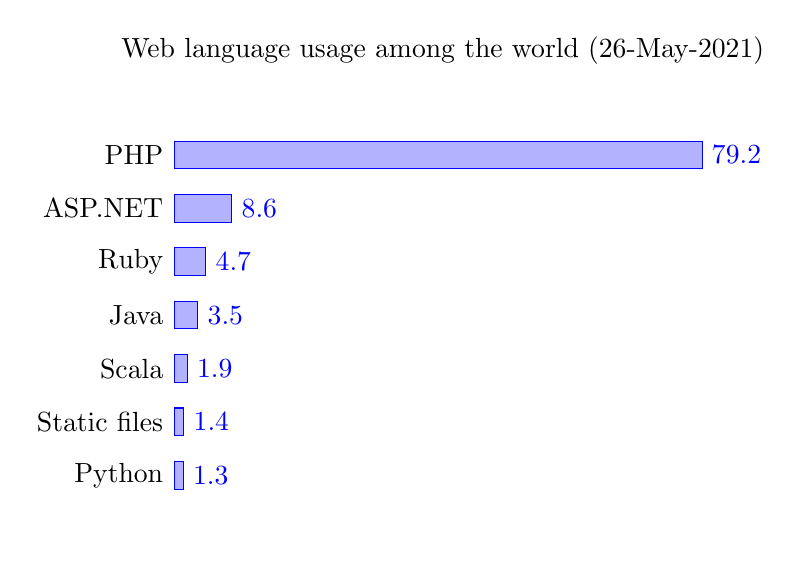
\begin{tikzpicture}
            \begin{axis}[title  = Web language usage among the world (26-May-2021),
                xbar,
                y axis line style = { opacity = 0 },
                axis x line       = none,
                tickwidth         = 0pt,
                ytick             = data,
                enlarge y limits  = 0.2,
                enlarge x limits  = 0.02,
                symbolic y coords = {Python, Static files, Scala, Java, Ruby, ASP.NET,  PHP},
                nodes near coords,
            ]
                \addplot coordinates { (79.2,PHP)         (8.6,ASP.NET)
                (4.7,Ruby)  (3.5,Java) (1.9,Scala) (1.4,Static files) (1.3,Python) };
            \end{axis}
        \end{tikzpicture}

        \url{https://w3techs.com/technologies/overview/programming_language}

        \subsubsection[Docker]{Docker}

        \begin{center}
            
\includegraphics[scale=0.3]{logo_docker}
        \end{center}

        \begin{flushleft}
            Regarding the docker decision, there wasn't much to think about, since docker is a modern technology which I
            already knew the bases, making it easier to pick up and start working earlier.
        \end{flushleft}

        \subsubsection[Docker-compose]{DockerCompose}

        \begin{center}
            
\includegraphics[scale=0.4]{logo_docker_compose}
        \end{center}

        \begin{flushleft}
            This tool facilitates deploying services on a server, while also being able to scalate the services or
            deploy them in a swarm, so there was no excuse to avoid its usage.
        \end{flushleft}

        \newpage
        \subsubsection[Portainer]{Portainer}

        \begin{center}
            
\includegraphics[scale=0.2]{logo_docker_portainer}
        \end{center}

        \begin{flushleft}
            Taking a look at different monitoring tools, decided to use docker portainer mainly by it's fast set-up.
            While still being up to the tasks demanded, which consist in monitoring and managing.
        \end{flushleft}

        \subsubsection[GitHub]{GitHub}

        \begin{center}
            
\includegraphics[scale=0.045]{logo_github}
        \end{center}

        \begin{flushleft}
            On the other hand, I decided to use GitHub to store the project mainly due having a basic understanding of how
            the tools work, since there are multiple tools that suits the same function, felt like that was the right decision.
        \end{flushleft}



        \newpage
        \subsubsection[PostgreSQL]{PostgresSQL}

        \begin{center}
            
\includegraphics[scale=0.3]{logo_postgresql}
        \end{center}

        \begin{flushleft}
            Meanwhile the web language was picked based on its global usage, I personally already have experience with
            Oracle, MySQL, MariaDB and MongoDB, so in order to try a different technology, I decided to use PostgreSQL,
            since it suited my needs while also learning a new database, yet, its position among the ranking, made the
            decision easier to take.
        \end{flushleft}

        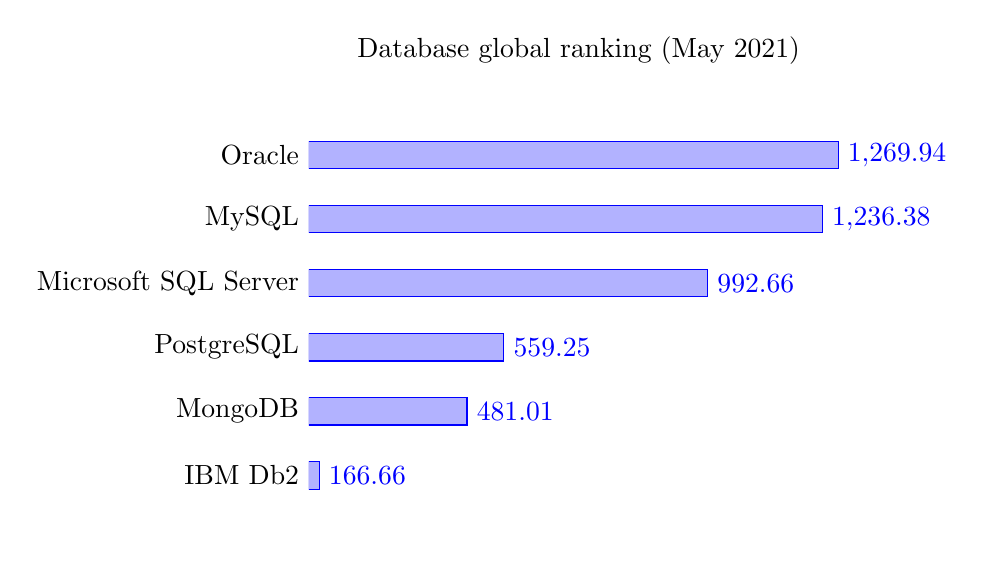
\begin{tikzpicture}
            \begin{axis}[title  = Database global ranking (May 2021),
            xbar,
            y axis line style = { opacity = 0 },
            axis x line       = none,
            tickwidth         = 0pt,
            ytick             = data,
            enlarge y limits  = 0.2,
            enlarge x limits  = 0.02,
            symbolic y coords = {IBM Db2, MongoDB, PostgreSQL, Microsoft SQL Server, MySQL,  Oracle},
            nodes near coords,
            ]
            \addplot coordinates { (1269.94,Oracle)         (1236.38,MySQL)
            (992.66 ,Microsoft SQL Server)  (559.25,PostgreSQL) (481.01,MongoDB) (166.66,IBM Db2) };
            \end{axis}
         \end{tikzpicture}

        \url{https://db-engines.com/en/ranking}

        \subsubsection[Nginx]{Nginx}

        \begin{center}
            
\includegraphics[scale=0.3]{logo_nginx}
        \end{center}
        \begin{flushleft}
            So far, being the main two options Apache and Nginx, I was quite limited when it came to variety,
            and yet, both suit its job very well, yet, due its minor differences, decided to use Nginx instead of Apache,
            since its less resource hungry while being more configurable-wise.
        \end{flushleft}

        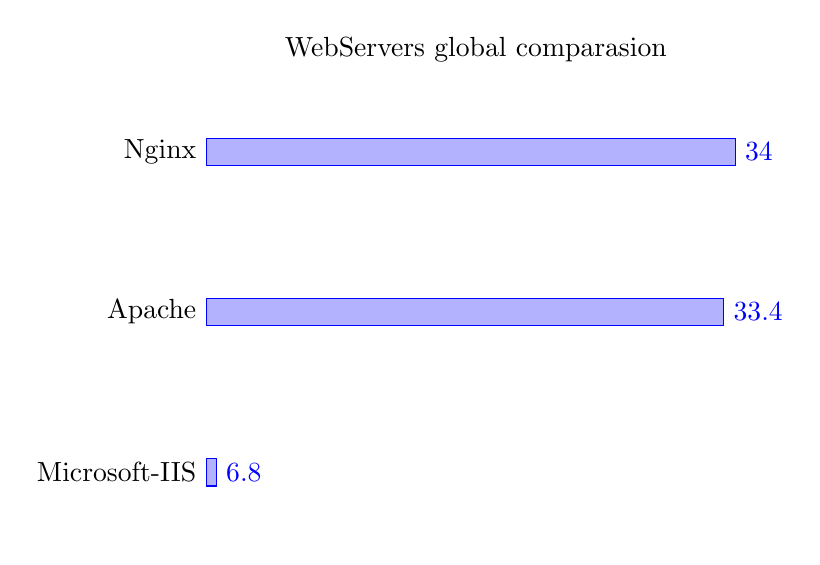
\begin{tikzpicture}
            \begin{axis}[title  = WebServers global comparasion,
            xbar,
            y axis line style = { opacity = 0 },
            axis x line       = none,
            tickwidth         = 0pt,
            ytick             = data,
            enlarge y limits  = 0.2,
            enlarge x limits  = 0.02,
            symbolic y coords = {Microsoft-IIS, Apache, Nginx},
            nodes near coords,
            ]
            \addplot coordinates { (34.0,Nginx) (33.4,Apache) (6.8 ,Microsoft-IIS)};
            \end{axis}
        \end{tikzpicture}

        \begin{flushleft}
            \url{https://w3techs.com/technologies/comparison/ws-apache,ws-microsoftiis,ws-nginx}
        \end{flushleft}

%    Project structure